% ========== CANADAGÅS ==========
\begin{frame}{%
  \begin{minipage}[c]{0.30\textwidth}
    Canadagås
  \end{minipage}%
  \hfill
  \begin{minipage}[c]{0.45\textwidth}
    \footnotesize
    \textbf{Jagttid:} 1.\ sep. -- 31.\ jan. samt 1.\ -- 31.\ aug.*
  \end{minipage}%
  \hfill
  \begin{minipage}[c]{0.15\textwidth}
    \noindent\raggedleft
    
\includegraphics[width=0.5cm, height=0.5cm, keepaspectratio]{Billeder/Ikoner/star.png}
  \end{minipage}%
}
  \vspace{0.25em}
  \begin{columns}[T]
    % --- Venstre kolonne: Tekst ---
    \column{0.45\textwidth}
    \setlength{\parskip}{0.5em}
    \tiny
    \RaggedRight
    \textbf{\textit{Branta canadensis}} – større hjemmehørende gås i rajgæs-familien \par
    \textbf{Udseende:}\\
    \quad – Stor krop og hvid plet bag øjet på kinden
    \par
    \textbf{* Jagttid 1. - 31. august:} \\
    \quad – \textbf{Krav} På arealer i omdrift (aktive marker/landbrug) med minimumsafstand på 300m til ferske vandre større end 3ha
    % --- Højre kolonne: Større billede ---
    \column{0.52\textwidth}
    \centering
    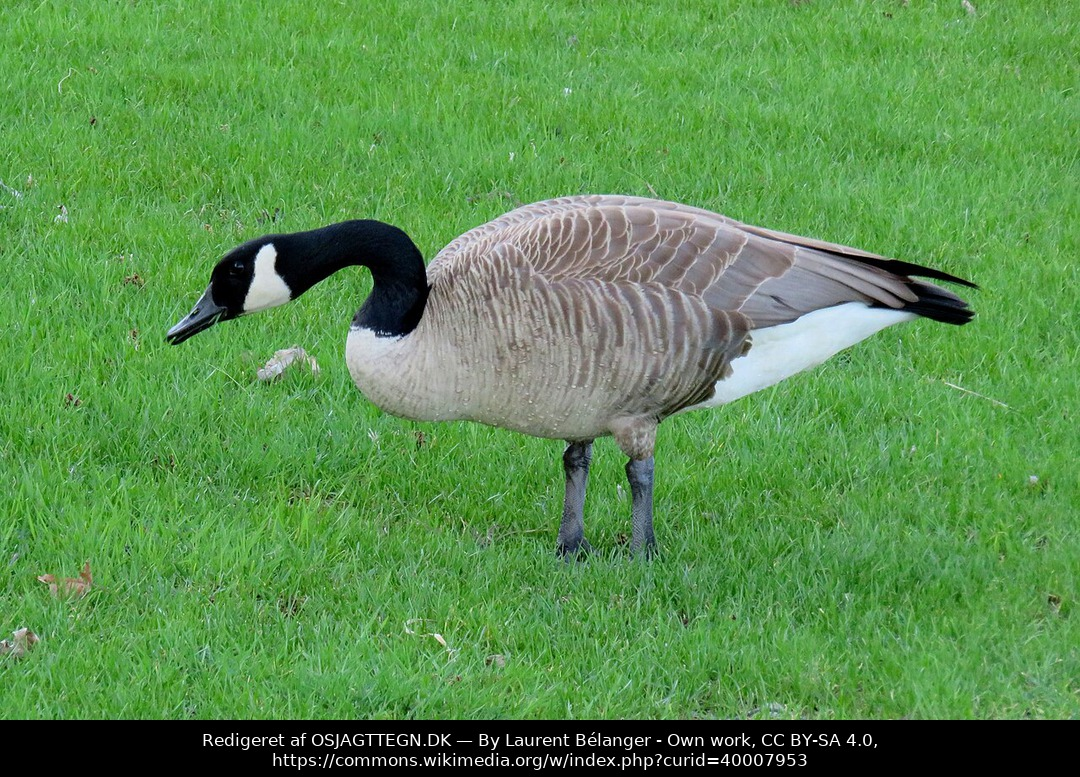
\includegraphics[width=\linewidth, height=7.2cm, keepaspectratio]{Billeder/Dyr/Fugle/Gaes/canadagås.jpg}
  \end{columns}
\end{frame}